% 拉格朗日点
% 限制性三体问题|拉格朗日点|旋转系等效势能

\pentry{限制性三体问题\upref{TriLim},雅可比常量\upref{JConst}}

对于大质量天体A和B围绕质心作匀速圆周运动的限制性三体问题,是否存在若干个特殊位置,使得处于该位置并满足一定的初始条件的第三质点将在运动中保持与天体A和B的相对位置不变,即第三质点同样围绕系统质心作匀速圆周运动,且角速度与天体A和B相同?这样的位置称为“\textbf{平动点}”或“\textbf{拉格朗日点}”

保持与天体A和B的相对位置不变,即要求第三质点在旋转坐标系中满足 $\dot{x}=\dot{y}=\dot{z}=\ddot{x}=\ddot{y}=\ddot{z}=0$,代入第三质点的动力学微分方程组(\autoref{JConst_eq2}\upref{JConst},\autoref{JConst_eq3}\upref{JConst} ,\autoref{JConst_eq4}\upref{JConst})可得方程组
\begin{align}
-\omega^2 x &=- \pdv{U}{x}=-\frac{\mu GM}{r_1^3}[x+(1-\mu)R]-\frac{(1-\mu)GM}{r_2^3}(x-\mu R)\label{LPoint_eq1}\\
-\omega^2 y &=- \pdv{U}{y}=-\qty[\frac{\mu GM}{r_1^3}+\frac{(1-\mu)GM}{r_2^3}]y\label{LPoint_eq2}\\
0 &=- \pdv{U}{z} =-\qty[\frac{\mu GM}{r_1^3}+\frac{(1-\mu)GM}{r_2^3}]z\label{LPoint_eq3}
\end{align}
观察\autoref{LPoint_eq3} 可得 $z=0$,即待求点在天体A、B的运动平面内.

若 $y=0$,则\autoref{LPoint_eq2} 恒成立.并且注意到A、B作匀速圆周运动时,根据外有引力等于向心力的关系,可得
\begin{equation}%4
\omega^2 =\frac{GM}{R^3}
\end{equation}
此时\autoref{LPoint_eq1} 便可化简为
\begin{equation}%5
\frac{x}{R^3} =\frac{\mu}{|x+(1-\mu)R|^3}[x+(1-\mu)R]+\frac{1-\mu}{|x-\mu R|^3}(x-\mu R)
\end{equation}
此方程没有解析解,只能借助数值方法求得其满足一定精度要求的数值解.可以验证在天体A、B之间及两边延长线方向上各有一个解,分别记为 $L_1,L_2,L_3$.

若 $y\neq 0$,则有
\begin{equation}%6
\leftgroup{
\frac{x}{R^3} &=\frac{\mu}{r_1^3}[x+(1-\mu)R]+\frac{1-\mu}{r_2^3}(x-\mu R)\\
\frac{1}{R^3} &=\frac{\mu}{r_1^3}+\frac{1-\mu}{r_2^3}
}
\end{equation}
解得 $r_1=r_2=R$,即平动点与A、B形成正三角形,这样的平动点有两个,分别记为 $L_4,L_5$.

拉格朗日点的力学本质是,第三质点在该位置所受的引力合力恰好等于维持匀速旋转所需的的向心力.五个拉格朗日点与A、B(在旋转坐标系内)的相对位置大致如\autoref{LPoint_fig1} 所示.
\begin{figure}[ht]
\centering
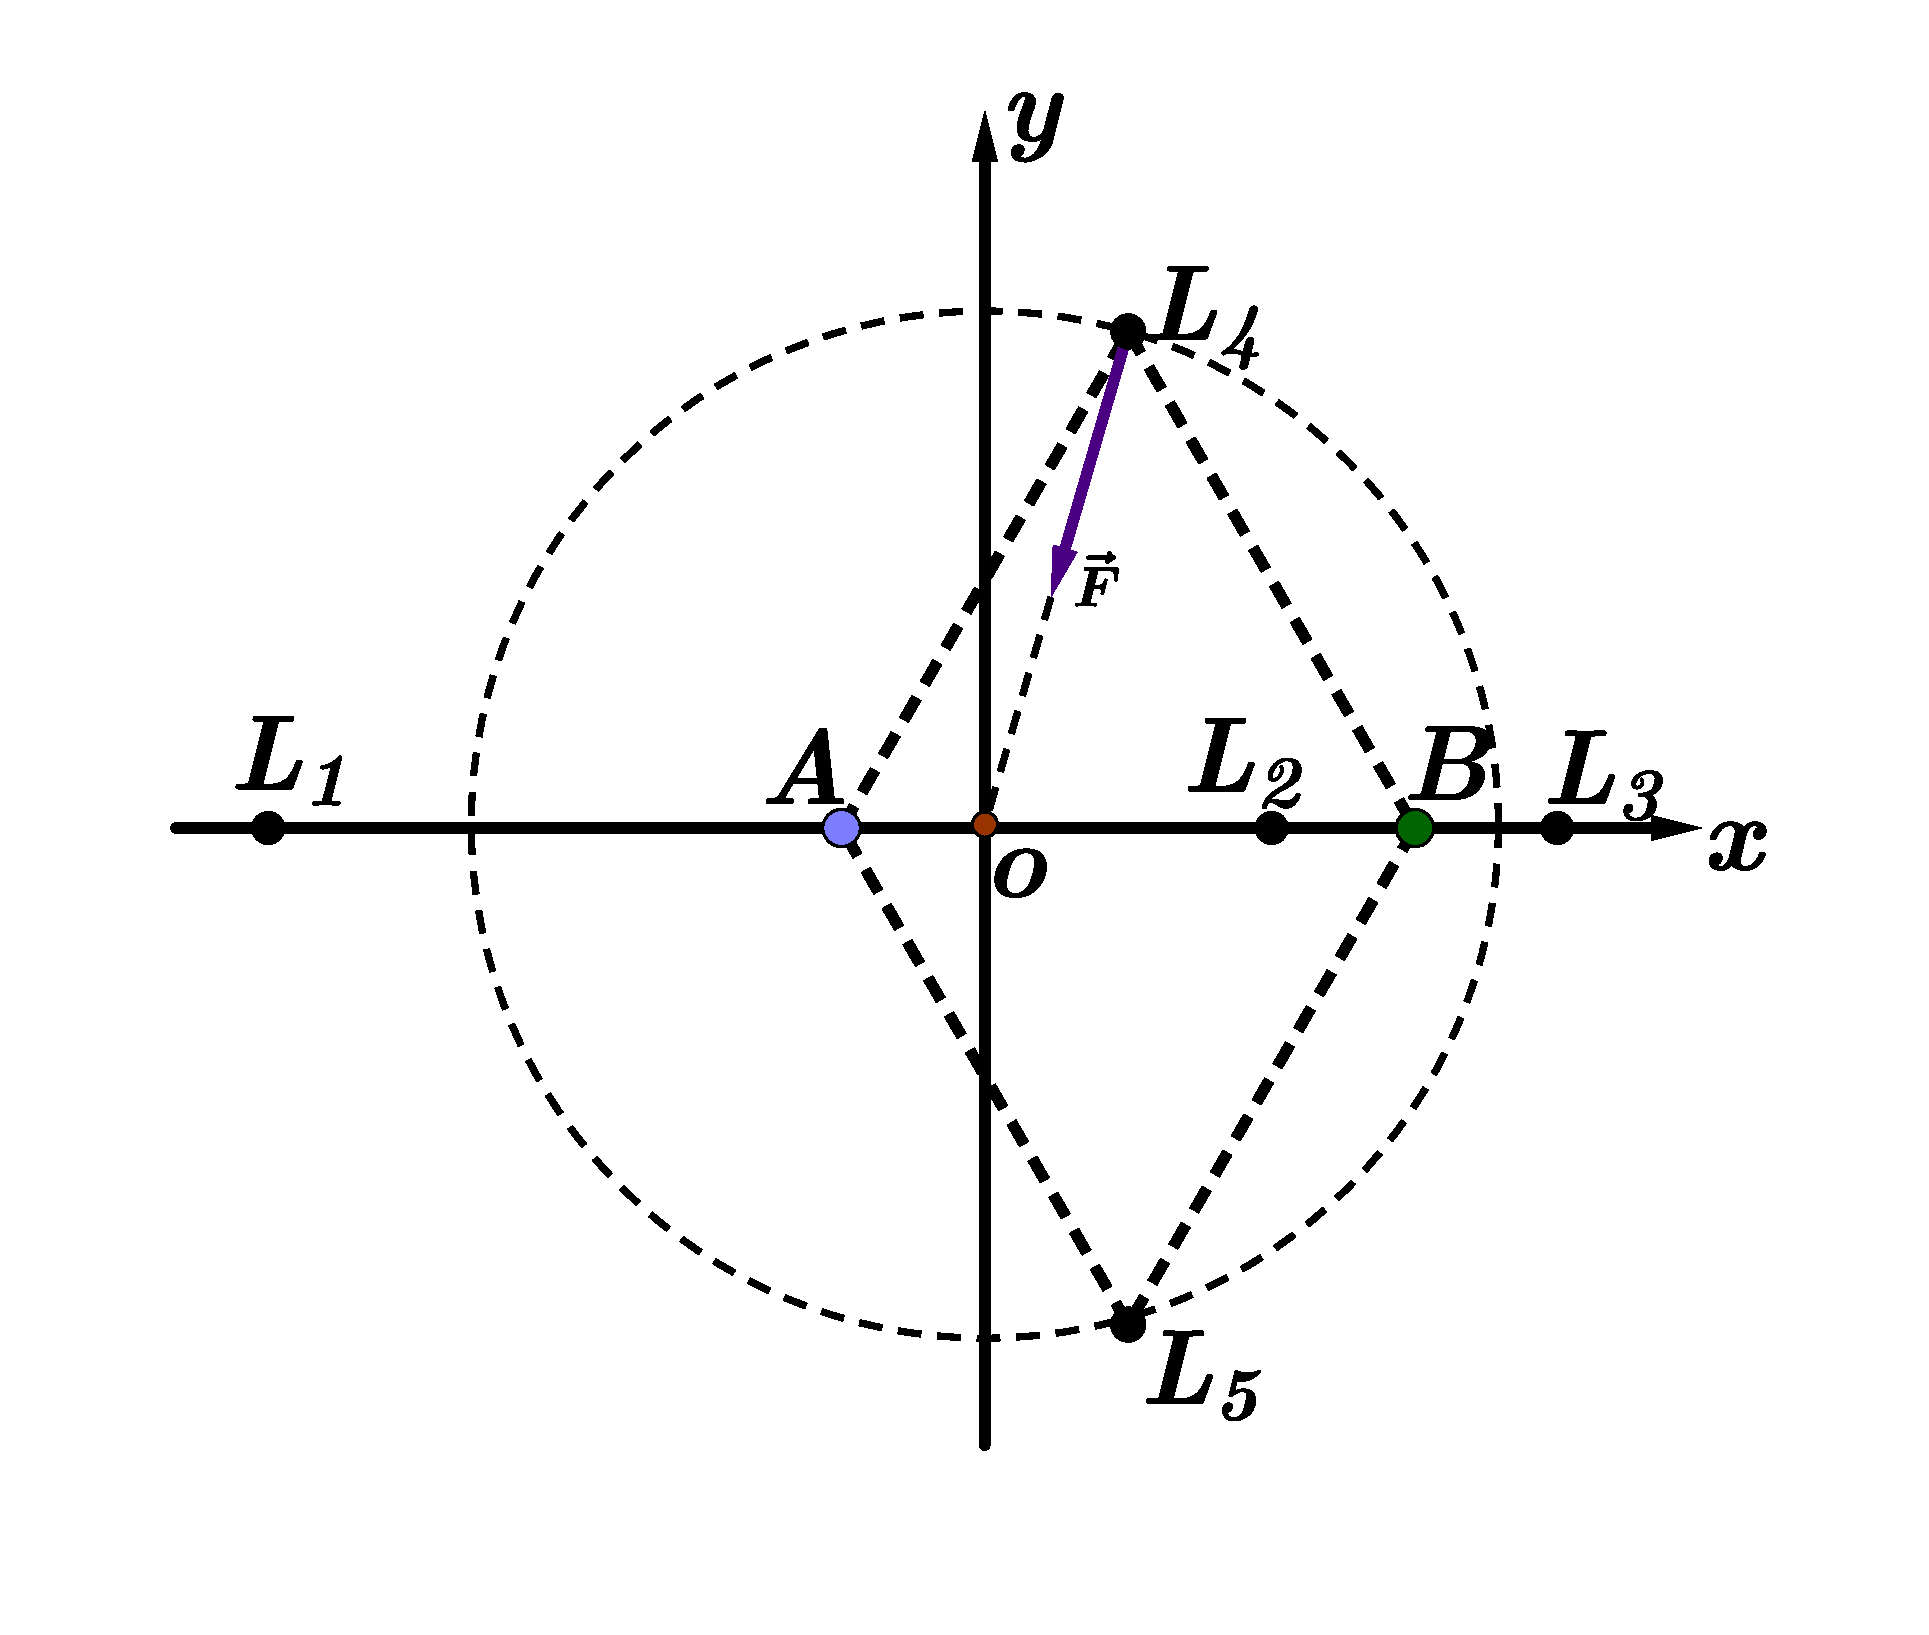
\includegraphics[width=8cm]{./figures/LPoint1.pdf}
\caption{拉格朗日点位置} \label{LPoint_fig1}
\end{figure}

\subsection{稳定性}
提取单位质量的雅可比常量(\autoref{JConst_eq12}\upref{JConst})中的势能部分,记为等效势能 $\widetilde{U}$ 
\begin{equation}%7
\widetilde{U}=-\frac{1}{2}\omega^2\qty(x^2+y^2)-\frac{\mu GM}{r_1}-\frac{(1-\mu) GM}{r_2}
\end{equation}
可见方程\autoref{LPoint_eq1},\autoref{LPoint_eq2} ,\autoref{LPoint_eq3} 等价于等效势能的一阶偏导数为零
 \begin{equation}%8
\pdv{\widetilde{U}}{x}=\pdv{\widetilde{U}}{y}=\pdv{\widetilde{U}}{z}=0
\end{equation}
等效势能在 $xoy$ 平面内部分区域的分布如\autoref{LPoint_fig2} 所示,图中A、B两点为等效势能的理论奇点,在其附近形成“势能陷阱”. 
\begin{figure}[ht]
\centering
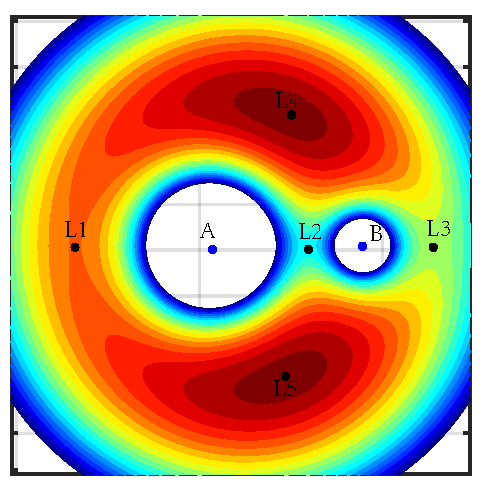
\includegraphics[width=8cm]{./figures/LPoint2.pdf}
\caption{等效势能的分布} \label{LPoint_fig2}
\end{figure}

一般而言,势能的极小值点为相对的稳定点.通过观察\autoref{LPoint_fig2} 可见,天体A、B连线上的 $L_1,L_2,L_3$ 三点附近的等势线呈形似“马鞍”的形状,处于这三点的质点C如果发生偏向A、B两者中任意一个天体的微小扰动,都会导致势能的快速减小,最终掉入“势能陷阱”.而 $L_4,L_5$ 虽然是势能的极大值点,但是由于其附近的等势线呈环形,并且势能变化平缓,处于此处的航天器发生微小扰动时,势能变化较小,只需消耗少量的燃料便可以遏制扰动的发散,因此 $L_4,L_5$ 是相对稳定的拉格朗日点.  


